
% This LaTeX was auto-generated from an M-file by MATLAB.
% To make changes, update the M-file and republish this document.

\documentclass{article}
\usepackage{graphicx}
\usepackage{color}

\sloppy
\definecolor{lightgray}{gray}{0.5}
\setlength{\parindent}{0pt}

\begin{document}

    
    
\section*{One-dimensional Conservation Law Solver}

\begin{par}
Computing Burgers solution using a DG-FEM routine with Polynomial truncation for the nonlinear terms.
\end{par} \vspace{1em}
\begin{par}
for solving the following problem:
\end{par} \vspace{1em}
\begin{par}
$u_t + f(u)_x = s(u)$
\end{par} \vspace{1em}
\begin{par}
where f(u) and S(u) can be For linear advection eq.: f(u) = a*u and s(u) = any function of u For non-linear advection: f(u) = u\^{}2/2 and s(u) = any function of u
\end{par} \vspace{1em}
\begin{par}
Function residual will be defined as:
\end{par} \vspace{1em}
\begin{par}
$Residue(u) = - f(u)_x + s(u)$
\end{par} \vspace{1em}
\begin{par}
Based on ideas of the following papers:
\end{par} \vspace{1em}
\begin{par}
1. TVB Runge-Kutta Local Projection Discontinuous Galerkin Finite Element Method for conservation laws II: General Framework. (1989) 2. Runge-Kutta Discontinuous Galerkin Method Using WENO Limiters. (2005)
\end{par} \vspace{1em}
\begin{par}
Coded by Manuel Diaz 2012.12.05
\end{par} \vspace{1em}

\subsection*{Contents}

\begin{itemize}
\setlength{\itemsep}{-1ex}
   \item Clear Work Space
   \item Simulation Parameters
   \item Define Grid Cell's (Global) nodes
   \item flux function
   \item Source term function
   \item SETUP
   \item Load Initial Condition, u(x,0) = u0
   \item Computing the evolution of the residue 'L(u)', du/dt = L(u)
   \item Write Output
\end{itemize}


\subsection*{Clear Work Space}

\begin{verbatim}
clear all; close all; clc;
\end{verbatim}


\subsection*{Simulation Parameters}

\begin{verbatim}
k         = 4;      % Space order / Number of degress of freedom: 0 to k
np        = k+1;    % Number of points per Cell/Element
quadn     = 3;      % element grid: {1}sLeg, {2}Lobatto, {3}Leg, {4}Radau
RKs       = 3;      % Time Int. Scheme {1} no-RK,  {2}TVD-RK2, {3}TVD-RK3,
                    %                  {4}SSP-RK2, {5}SSP-RK3, {6}SSP-RK4S5
flux_type = 3;      % {1}Roe, {2}Global LF, {3}LLF, {4}Upwind (non-conservative)
equation  = 2;      % {1} scalar advection, {2} burgers equation
include_s = 0;      % {1} include source term, {0} do NOT include source term
a         = 1.0;    % for scalar advection speed
cfl       = 1/(2*k+1);    % Courant Number
tEnd      = 3.10;   % Final Time for computation
nx        = 10;     % Number of Cells/Elements
MM        = 0.01;   % TVB constant M
IC_case   = 3;      % {1} Gaussian , {2} Square, {3} sine, {4} Riemann.
plot_figs = 1;      % {1}Plot figures, {0}Do NOT plot figures
w_output  = 0;      % Write output: {1} YES please!, {2} NO
\end{verbatim}


\subsection*{Define Grid Cell's (Global) nodes}

\begin{par}
Building nodes for cells/elements:
\end{par} \vspace{1em}
\begin{verbatim}
x_left = 0; x_right = 1; dx = (x_right-x_left)/nx;
x_nodes = x_left : dx : x_right; % cells nodes
\end{verbatim}


\subsection*{flux function}

\begin{verbatim}
switch equation
    case{1} % Scalar advection Eq. flux:
        F  = @(w) a * w;
        % and derivate of the flux function
        dF = @(w) a*ones(size(w));
    case{2} % Invicied Burgers Eq. flux:
        F  = @(w) w.^2/2;
        % and derivate of the flux function
        dF = @(w) w;
end
\end{verbatim}


\subsection*{Source term function}

\begin{verbatim}
switch include_s
    case{0} % no source term
        S = @(w) zeros(size(w));
    case{1} % with source term
        % example source term
        S = @(w) w.^2;
end
\end{verbatim}


\subsection*{SETUP}

\begin{par}
1. Build Cells/Elements (Local) inner points (quadrature points). 2. Build Weigthing values for our local. 3. Build Vandermonde Matrix for our local quadrature points.
\end{par} \vspace{1em}
\begin{verbatim}
[x,xi,w,V] = setup(k,x_nodes,quadn);

% Compute Math Objetcs:
if quadn == 1; bmath = 1; else bmath = 2; end;
switch bmath
    case{1} % Build Math objects for scaled Legendre polynomials. See Ref.[1]
        % M matrix
        Mcoef = [1 1/12 1/180 1/2800 1/44100 1/698544 1/11099088 1/176679360];
        M = diag(Mcoef(1:k+1));
        % invM matrix
        invM = inv(M);
        % D matrix
        Dcoef = [ ...
            0, 1, 0, (1/10), 0, (1/126), 0, (1/1716); ...
            0, 0, (1/6), 0, (1/70), 0, (1/924), 0; ...
            0, 0, 0, (1/60), 0, (1/756), 0, (1/10296); ...
            0, 0, 0, 0, (1/700), 0, (1/9240), 0; ...
            0, 0, 0, 0, 0, (1/8820), 0, (1/120120); ...
            0, 0, 0, 0, 0, 0, (1/116424), 0; ...
            0, 0, 0, 0, 0, 0, 0, (1/1585584); ...
            0, 0, 0, 0, 0, 0, 0, 0];
        D = Dcoef(1:k+1,1:k+1);
        % Scaled Legendre polynomials of deg 'l' evaluated at x = +1/2
        Ln = zeros(k+1,1); % column vector
        for l = 0:k; % Polynomials degree
        Ln(l+1) = sLegendreP(l,0.5);
        end
        % Scaled Legendre polynomials of deg 'l' evaluated at x = -1/2
        Lp = zeros(k+1,1); % column vector
        for l = 0:k; % Polynomials degree
        Lp(l+1) = sLegendreP(l,-0.5);
        end

    case{2} % Build Math objects for non-scaled Legendre polynomials See Ref.[3]
    l = (0:k)'; % all polynomials degree
    % M matrix
    M = diag(dx./(2*l+1));
    % invM matrix
    invM = inv(M);
    % D matrix
    D = zeros(np,np);
    for ll = 0:k            % For all degress of freedom
        i = ll+1;           % Dummy index
        for j=1:np          % For all local points
            if j>i && rem(j-i,2)==1
                D(i,j)=2;   % D or diffentiated Legendre Matrix
            end
        end
    end
    % Scaled Legendre polynomials of degree 'l' evaluated at x = +1
    Ln = (1).^(l);  % LegP @ x_{i+1/2}^(-)
    % Scaled Legendre polynomials of degree 'l' evaluated at x = -1
    Lp = (-1).^(l); % LegP @ x_{i-1/2}^(+)
end
\end{verbatim}


\subsection*{Load Initial Condition, u(x,0) = u0}

\begin{verbatim}
u0 = u_zero(x,IC_case);
f0 = F(u0);
s0 = S(u0);
\end{verbatim}


\subsection*{Computing the evolution of the residue 'L(u)', du/dt = L(u)}

\begin{par}
Load Initial conditions
\end{par} \vspace{1em}
\begin{verbatim}
u = u0;

% Transform u(x,t) to degress of freedom u(t)_{l,i} for each i-Cell/Element
ut = V\u;

% Set Initial time step
t = 0; % time
n = 0; % counter
tic;
while t <= tEnd
    % Time step 'dt'
    u_reshaped = reshape(u,1,nx*np);
    dt  = dx*cfl/max(abs(u_reshaped));
    t  = t + dt;   % iteration time / increment time
    n  = n + 1;    % update counter

    % Plot solution every time step
    if plot_figs == 1; plot(x,u,'o-');
        title('u_t + f(u)_x = s(u)')
        xlabel('x'); ylabel('u')
        grid on; %axis([0,1,-5,5]);
    end;

    switch RKs % time integration scheme
        case{1} % no integration scheme
            ut_next = ut + dt*AdvecResidue(ut...
                ,F,dF,S,Ln,Lp,V,D,invM,flux_type);

        case{2} % TVD-RK2
            ut_1 = ut + dt*AdvecResidue(ut...
                ,F,dF,S,Ln,Lp,V,D,invM,flux_type);
            ut_next = 1/2*ut + 1/2*ut_1 + 1/2*dt*AdvecResidue(ut_1 ...
                ,F,dF,S,Ln,Lp,V,D,invM,flux_type);

        case{3} % TVD-RK3
            ut_1 = ut + dt*AdvecResidue(ut ...
                ,F,dF,S,Ln,Lp,V,D,invM,flux_type);
            ut_2 = 3/4*ut + 1/4*ut_1 + 1/4*dt*AdvecResidue(ut_1 ...
                ,F,dF,S,Ln,Lp,V,D,invM,flux_type);
            ut_next = 1/3*ut + 2/3*ut_2 + 2/3*dt*AdvecResidue(ut_2 ...
                ,F,dF,S,Ln,Lp,V,D,invM,flux_type);

        case{4} % 2nd Order SSP-RK
            u_1 = u + dt*residual(u,t);
            u_next = 1/2*(u + u_1 + dt*residual(u_1,t+dt));

        case{5} % 3rd Order SSP-RK
            u_1 = u + dt*residual(u,t);
            u_2 = 1/4*(3*u + u_1 + dt*residual(u_1,t+dt));
            u_next = 1/3*(u + 2*u_2 + 2*dt*residual(u_2,t+0.5*dt));

        case{6} % 5-stages, 4th-order SSP-RK
            % "It is not possible to construc a fourth-order, four-stage
            % SSP-RK schemes where all coefficients are positive." [3]
            % However, one can derive a fourth-order scheme by allowing a
            % fifth stage. The optimal scheme is given as:
            %
            % Low storage Runge-Kutta coefficients
            rk4a = [            0.0 ...
                    -567301805773.0/1357537059087.0 ...
                    -2404267990393.0/2016746695238.0 ...
                    -3550918686646.0/2091501179385.0  ...
                    -1275806237668.0/842570457699.0];
            rk4b = [ 1432997174477.0/9575080441755.0 ...
                     5161836677717.0/13612068292357.0 ...
                     1720146321549.0/2090206949498.0  ...
                     3134564353537.0/4481467310338.0  ...
                     2277821191437.0/14882151754819.0];
            rk4c = [             0.0  ...
                     1432997174477.0/9575080441755.0 ...
                     2526269341429.0/6820363962896.0 ...
                     2006345519317.0/3224310063776.0 ...
                     2802321613138.0/2924317926251.0];
            resu = 0;
            for s = 1:5
                timelocal = t + rk4c(s)*dt;
                [rhsu] = residual(u,timelocal);
                resu = rk4a(s)*resu + dt*rhsu;
                u = u + rk4b(s)*resu;
            end
            u_next = u;

        otherwise
            error ('Scheme not defined')
    end

    % UPDATE info
    ut = ut_next;

    % Update plot
    drawnow

    % Transform degress u(t)_{l,i} into values u(x,t)
    u = V*ut;

end % time loop
toc;
\end{verbatim}

        \color{lightgray} \begin{verbatim}Elapsed time is 2.390232 seconds.
\end{verbatim} \color{black}
    
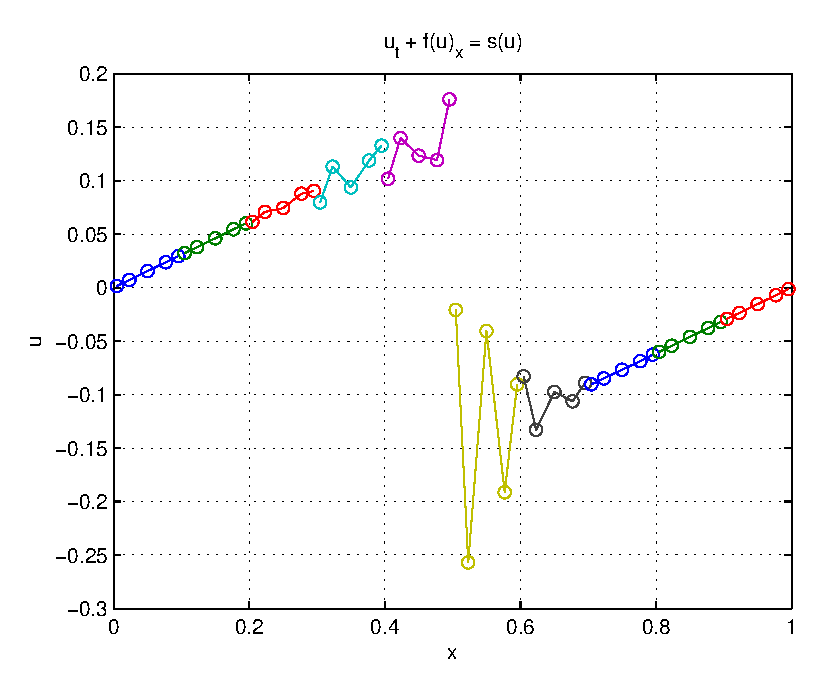
\includegraphics [width=4in]{DGFEM_RK_01.eps}


\subsection*{Write Output}

\begin{par}
Write output to tecplot
\end{par} \vspace{1em}
\begin{verbatim}
if w_output == 1;
    % write to tecplot subroutine
end;
\end{verbatim}



\end{document}
    
